% vim:autoindent:set textwidth=78:

\section{Características de un vistazo}\label{feature_glance}

% when the revision of a section has been finalized, 
% comment out the following line:
%\updatedisclaimer

Después de una primera y sencilla sesión en la Sección \ref{label_getstarted}, ahora
queremos mostrarle una ojeada más detallada de las características de QGIS. 
La mayoría de las características presentadas en los siguientes capítulos se explicarán
y describirán en sus propias secciones más adelante en el manual.

\subsection{Iniciar y detener QGIS}\label{label_startinqgis}

En la Secciónn \ref{samplesession} ya aprendió como iniciar QGIS. Repetiremos
esto aquí y verá que QGIS también proporciona más opciones de línea de órdenes. 

\begin{itemize}
\item \nix{suponiendo que tiene QGIS instalado en el PATH, puede iniciar QGIS
tecleando: \usertext{qgis} en la línea de órdenes o haciendo doble clic sobre el enlace a QGIS 
(o acceso directo) del escritorio.}
\item \win{inicie QGIS usando el menú Inicio o un acceso directo del escritorio, 
o haga doble clic en un archivo de proyecto de QGIS.}
\item \osx{doble clic en el icono de la carpeta Aplicaciones.}
\end{itemize} 

Para detener QGIS, pulse las opciones de menú \{\nix{}\win{Archivo} \osx{QGIS}\} > Salir,
o use el atajo de teclado \keystroke{Ctrl+Q}.

\subsubsection{Opciones de línea de órdenes}\index{command line options}
\label{label_commandline}

\nix QGIS admite un buen número de opciones cuando se inicia desde la línea de 
órdenes. Para obtener la lista de opciones, teclee \usertext{qgis ---help} en la
línea de órdenes.
La sentencia de uso para QGIS es:

\small
\begin{verbatim}
qgis --help
Quantum GIS - 1.1.0-Pan (Unstable) 'Pan (Unstable)'
Quantum GIS (QGIS) is a viewer for spatial data sets, including
raster and vector data.
Usage: qgis [options] [FILES]
  options:
        [--snapshot filename]   emit snapshot of loaded datasets to given file
        [--lang language]       use language for interface text
        [--project projectfile] load the given QGIS project
        [--extent xmin,ymin,xmax,ymax]  set initial map extent
        [--help]                this text

  FILES:
    Files specified on the command line can include rasters,
    vectors, and QGIS project files (.qgs):
     1. Rasters - Supported formats include GeoTiff, DEM
        and others supported by GDAL
     2. Vectors - Supported formats include ESRI Shapefiles
        and others supported by OGR and PostgreSQL layers using
        the PostGIS extension
\end{verbatim}
\normalsize

\begin{Tip} \caption{\textsc{Ejemplo utilizando argumentos en línea de órdenes}}
\qgistip{Puede iniciar QGIS especificando uno o más archivos de datos sobre la
línea de órdenes. Por ejemplo, suponiendo que está en el directorio 
qgis\_sample\_data, podría iniciar QGIS con una capa vectorial 
y un archivo ráster preparados para cargarlos 
en el arranque utilizando la siguiente orden: 
\usertext{qgis ./raster/landcover.img ./gml/lakes.gml}
}
\end{Tip}

\minisec{Opción de línea de órdenes \usertext{---snapshot}}
Esta opción permite crear una captura de pantalla en formato PNG de la vista actual.
Esto puede ser útil cuando se tienen muchos proyectos y se quieren generar capturas de los datos.

Actualmente esto genera un fichero PNG con 800x600 píxeles. Se puede añadir un nombre después de
\usertext{---snapshot}.

\minisec{Opción de línea de órdenes \usertext{---lang}}
En base a su configuración local, QGIS selecciona la localización correcta. Si se quiere 
cambiar el idioma, se puede especificar el código del idioma. Por ejemplo:
\usertext{---lang=it}
arranca QGIS con la localización en italiano. En \url{http://wiki.qgis.org/qgiswiki/TranslatorsCorner}
se proporciona una lista de los idiomas admitidos actualmente con su código.

\minisec{Opción de línea de órdenes \usertext{---project}}
También es posible iniciar QGIS con un proyecto existente. Simplemente añada 
la opción \usertext{---project} seguida del nombre de su proyecto y QGIS se abrirá 
con todas las capas cargadas definidas en el fichero dado.

\minisec{Opción de línea de órdenes \usertext{---extent}}
Para arrancar con una extensión específica del mapa utilice esta opción. Es necesario
añadir los límites en el siguiente orden separados por comas:
\begin{verbatim}
--extent xmin,ymin,xmax,ymax
\end{verbatim}


\subsection{Interfaz Gráfica de Usuario (GUI) de QGIS}\index{main window}
\label{label_qgismainwindow}

Cuando QGIS arranca, se encuentra con la GUI como se muestra abajo
(los números del 1 hasta el 6 en ovalos amarillos señalan las seis áreas principales 
de la interfaz que se describen abajo):

\begin{figure}[ht]
   \begin{center}
   \caption{Interfaz de QGIS con datos de ejemplo de Alaska \nixcaption}
	 \label{fig:startup}
   \includegraphics[clip=true, width=17cm]{startup}
\end{center} 
\end{figure}

\textbf{Nota:} La decoración de su ventana (barra de título, etc.) puede aparecer 
distinta dependiendo del sistema operativo y administrador de ventanas.

La Interfaz Gráfica de Usuario (GUI) de QGIS está dividida en seis áreas:

\begin{tabbing}
1. Barra de menús \hspace{3cm}\= 4. Vista del mapa \\
2. Barra de herramientas \hspace{3cm}\> 5. Vista general del mapa \\
3. Capas \hspace{3cm}\> 6. Barra de estado   
\end{tabbing}

Estos seis componentes de la interfaz de QGIS se describen con más detalle
en las siguientes secciones.

\subsubsection{Barra de menús}\label{label_menubar}
\index{menus}

La barra de menús proporciona acceso a varias características de QGIS utilizando 
menús jerárquicos estándar. A continuación se lista el nivel superior de los menús
y un resumen de algunas opciones de menú, junto con los iconos de las herramientas
correspondientes tal como aparece en la barra de herramientas, así como atajos de
teclado. Aunque la mayoría de opciones de menú tiene una herramientas y viceversa,
los menús no están organizados igual que las barras de herramientas. La barra de
herramientas que contiene cada herramienta se indica después de cada opción de menú
como una casilla de verificación. Para más información sobre herramientas y barras
de herramientas, vea la Sección \ref{label_toolbars}.

\begin{tabbing}
\hspace{6.5cm}\=\hspace{3cm}\=\hspace{3.5cm}\= \kill
\hspace{1cm} Opción de menú \> Atajo \> Referencia \> Barra de herramientas\\
\end{tabbing}

\begin{itemize}
\item \mainmenuopt{Archivo}
\begin{tabbing}
\hspace{5.5cm}\=\hspace{3cm}\=\hspace{3.5cm}\= \kill
\dropmenuopttwo{mActionFileNew}{Nuevo proyecto}
	\> \keystroke{Ctrl+N}
	\> Ver sección \ref{sec:projects}
	\> \dropmenucheck{Archivo} \\
\dropmenuopttwo{mActionFileOpen}{Abrir proyecto}
	\> \keystroke{Ctrl+O}
	\> Ver sección \ref{sec:projects}
	\> \dropmenucheck{Archivo} \\
\dropmenuopt{Abrir proyectos recientes}
	\>
	\> Ver sección \ref{sec:projects} \\
\dropmenuopttwo{mActionFileSave}{Guardar proyecto}
	\> \keystroke{Ctrl+S}
	\> Ver sección \ref{sec:projects}
	\> \dropmenucheck{Archivo} \\
\dropmenuopttwo{mActionFileSaveAs}{Guardar proyecto como}
	\> \keystroke{Ctrl+Shift+S}
  \> Ver sección \ref{sec:projects}
	\> \dropmenucheck{Archivo} \\
\dropmenuopttwo{mActionSaveMapAsImage}{Guardar como imagen}
	\>
	\> Ver sección \ref{sec:output} \\
\dropmenuopttwo{mActionFilePrint}{Diseñador de impresión}
	\> \keystroke{Ctrl+P}
	\> Ver sección \ref{label_printcomposer}
	\> \dropmenucheck{Archivo} \\
\dropmenuopttwo{mActionFileExit}{Salir} 
	\> \keystroke{Ctrl+Q} \\
\end{tabbing}

\item \mainmenuopt{Edición}
\begin{tabbing}
\hspace{5.5cm}\=\hspace{3cm}\=\hspace{3.5cm}\= \kill
\dropmenuopttwo{mActionEditCut}{Cortar objetos espaciales} 
	\> \keystroke{Ctrl+X}
	\> Ver sección \ref{sec:edit_existing_layer} 
	\> \dropmenucheck{Digitalización} \\
\dropmenuopttwo{mActionEditCopy}{Copiar objetos espaciales}
	\> \keystroke{Ctrl+C}
	\> Ver sección \ref{sec:edit_existing_layer} 
	\> \dropmenucheck{Digitalización} \\
\dropmenuopttwo{mActionEditPaste}{Pegar objetos espaciales} 
	\> \keystroke{Ctrl+V}
	\> Ver sección \ref{sec:edit_existing_layer} 
	\> \dropmenucheck{Digitalización} \\
\dropmenuopttwo{mActionCapturePoint}{Añadir punto}
	\> \keystroke{.}
	\> Ver sección \ref{sec:edit_existing_layer} 
	\> \dropmenucheck{Digitalización} \\
\dropmenuopttwo{mActionCaptureLine}{Añadir línea}
	\> \keystroke{/}
	\> Ver secciónn \ref{sec:edit_existing_layer} 
	\> \dropmenucheck{Digitalización} \\
\dropmenuopttwo{mActionCapturePolygon}{Añadir polígono}
	\> \keystroke{Ctrl+/}
	\> Ver sección \ref{sec:edit_existing_layer} 
	\> \dropmenucheck{Digitalización} \\
Y otros elementos del menú Edición
	\>
	\> Ver sección \ref{sec:edit_existing_layer} 
	\> \dropmenucheck{Digitalización} \\
%\dropmenuopt{Move Feature}
%	\> \> \dropmenucheck{Edit} \\
%\dropmenuopt{Split Features}
%	\> \> \dropmenucheck{Edit} \\
%\dropmenuopt{Delete Selected}
%	\> \> \dropmenucheck{Edit} \\
%\dropmenuopt{Add Vertex}
%	\> \> \dropmenucheck{Edit} \\
%\dropmenuopt{Move Vertex}
%	\> \> \dropmenucheck{Edit} \\
%\dropmenuopt{Delete Vertex}
%	\> \> \dropmenucheck{Edit} \\
%\dropmenuopt{Add Ring}\footnote{New since v0.9} 
%	\>
%	\> \dropmenucheck{Edit} \\
%\dropmenuopt{Add Island} \footnotemark[\value{footnote}] 
%	\>
%	\> \dropmenucheck{Edit} \\
\end{tabbing}


\item \mainmenuopt{Ver}
\begin{tabbing}
\hspace{5.5cm}\=\hspace{3cm}\=\hspace{3.5cm}\= \kill
\dropmenuopttwo{mActionPan}{Desplazar mapa}
	\>
	\> \> \dropmenucheck{Navegación de mapas} \\
\dropmenuopttwo{mActionZoomIn}{Acercar zum}
	\> \keystroke{Ctrl++}
	\> \> \dropmenucheck{Navegación de mapas} \\
\dropmenuopttwo{mActionZoomOut}{Alejar zum}
	\> \keystroke{Ctrl+-}
	\> \> \dropmenucheck{Navegación de mapas} \\
\dropmenuopttwo{mActionSelect}{Seleccionar objetos espaciales}
	\>
	\> \> \dropmenucheck{Atributos} \\
\dropmenuopttwo{mActionIdentify}{Identificar objetos espaciales}
	\> \keystroke{I}
	\> \> \dropmenucheck{Atributos} \\
\dropmenuopttwo{mActionMeasure}{Regla}
	\> \keystroke{M}
	\> \> \dropmenucheck{Atributos} \\
\dropmenuopttwo{mActionMeasureArea}{Medir áreas}
	\> \keystroke{J}
	\> \> \dropmenucheck{Atributos} \\
\dropmenuopttwo{mActionOpenTable}{Zum general}
	\> \keystroke{F}
	\> \> \dropmenucheck{Navegación de mapas} \\
\dropmenuopttwo{mActionZoomToLayer}{Zum a la capa}
	\>
	\> \> \dropmenucheck{Navegación de mapas} \\
\dropmenuopttwo{mActionZoomToSelected}{Zum a la selección}
	\> \keystroke{Ctrl+J}
	\> \> \dropmenucheck{Navegación de mapas} \\
\dropmenuopttwo{mActionZoomLast}{Zum anterior}
	\>
		\> \> \dropmenucheck{Navegación de mapas} \\
\dropmenuopttwo{mActionZoomNext}{Zum siguiente}
	\>
	\> \> \dropmenucheck{Navegación de mapas} \\
\dropmenuopt{Zum al tamaño real}
	\>
	\> \>  \\
\dropmenuopttwo{mActionMapTips}{Avisos del mapa}
	\>
	\> \> \dropmenucheck{Atributos} \\
\dropmenuopttwo{mActionNewBookmark}{Nuevo marcador}
	\> \keystroke{Ctrl+B}
	\> Ver sección \ref{sec:bookmarks} 
\> \dropmenucheck{Atributos} \\
\dropmenuopttwo{mActionShowBookmarks}{Mostrar marcadores}
	\> \keystroke{B}
	\> Ver sección \ref{sec:bookmarks} 
	\> \dropmenucheck{Atributos} \\
\dropmenuopttwo{mActionDraw}{Actualizar}
	\> \keystroke{Ctrl+R}
	\> \> \dropmenucheck{Navegación de mapas} \\
\end{tabbing}

\item \mainmenuopt{Capa}
\begin{tabbing}
\hspace{5.5cm}\=\hspace{3cm}\=\hspace{3.5cm}\= \kill
\dropmenuopttwo{mActionNewVectorLayer}{Nueva capa vectorial}
	\> \keystroke{N}
	\>          	
	Ver sección \ref{sec:create shape}
	\> \dropmenucheck{Administrar capas} \\
\dropmenuopttwo{mActionAddNonDbLayer}{Añadir capa vectorial}       
	\> \keystroke{V}
	\>          	
	Ver sección \ref{label_workingvector}
	\> \dropmenucheck{Archivo} \\
\dropmenuopttwo{mActionAddRasterLayer}{Añadir capa ráster}       
	\> \keystroke{R}
	\>          	
	Ver sección \ref{label_raster}
	\> \dropmenucheck{Archivo} \\
\dropmenuopttwo{mActionAddLayer}{Añadir capa PostGIS}      
	\> \keystroke{D}
	\>          	
	Ver sección \ref{label_postgis}
	\> \dropmenucheck{Archivo} \\
\dropmenuopttwo{mActionAddWmsLayer}{Añadir capa WMS}          
	\> \keystroke{W}
	\>          	
	Ver sección \ref{sec:ogc-wms}
	\> \dropmenucheck{Archivo} \\
\dropmenuopttwo{mActionOpenTable}{Abrir tabla de atributos}
	\> \>
	\> \dropmenucheck{Atributos} \\
\dropmenuopttwo{mActionToggleEditing}{Conmutar edición}
	\> \>
	\> \dropmenucheck{Digitalización} \\
\dropmenuopt{Guardar como archivo shape}
	\\
\dropmenuopt{Guardar la selección como archivo shape}
	\\
\dropmenuopttwo{mActionRemoveLayer}{Eliminar capa}
	\> \keystroke{Ctrl+D}
	\>          	
	\> \dropmenucheck{Administrar capas} \\
\dropmenuopt{Propiedades}
	\\
\dropmenuopttwo{mActionInOverview}{Añadir a la vista general}
	\> \keystroke{O}
	\>          	
	\> \dropmenucheck{Administrar capas} \\
\dropmenuopttwo{mActionAddAllToOverview}{Añadir todo a la vista general}
	\> \keystroke{+}
	\>          	
	\\
\dropmenuopttwo{mActionRemoveAllFromOverview}{Eliminar todo de la vista general}
	\> \hspace{1cm}\keystroke{-}
	\>          	
	\\
\dropmenuopttwo{mActionHideAllLayers}{Ocultar todas las capas}
	\> \keystroke{H}
	\>          	
	\> \dropmenucheck{Administrar capas} \\
\dropmenuopttwo{mActionShowAllLayers}{Mostrar todas las capas}
	\> \keystroke{S}
	\>          	
	\> \dropmenucheck{Administrar capas} \\
\end{tabbing}

\item \mainmenuopt{Configuración}
\begin{tabbing}
\hspace{5.5cm}\=\hspace{3cm}\=\hspace{3.5cm}\= \kill
\dropmenuopt{Paneles}  
	\>           
	\>          	
	\\
\dropmenuopt{Barras de herramientas}  
	\>           
	\>          	
	\\
\dropmenuopt{Conmutar el modo de pantalla completa}  
	\>
	\>          	
	\\
\dropmenuopttwo{mActionProjectProperties}{Propiedades del proyecto}  
	\> \keystroke{P}
	\>          	
	Ver sección \ref{sec:projects}
	\\
\dropmenuopttwo{mActionCustomProjection}{SRC personalizado}   
\> \>          	
Ver sección \ref{sec:customprojections}
	\\
\dropmenuopttwo{mActionOptions}{Opciones}             
\> \>          	
Ver sección \ref{subsec:gui_options}
	\\
\end{tabbing}

\item \mainmenuopt{Complementos} - (Se añaden más elementos de menú a medida que se cargan complementos.)
\begin{tabbing}
\hspace{5.5cm}\=\hspace{3cm}\=\hspace{3.5cm}\= \kill
\dropmenuopttwo{mActionShowPluginManager}{Administrador de complementos}          	   
\> \>          	
Ver sección \ref{sec:managing_plugins}
	\dropmenucheck{Complementos}\\
\end{tabbing}          	

\item \mainmenuopt{Ayuda}
\begin{tabbing}
\hspace{5.5cm}\=\hspace{3cm}\=\hspace{3.5cm}\= \kill
\dropmenuopttwo{mActionHelpContents}{Contenidos de la ayuda}
	\> \keystroke{F1}
	\>           	
	\> \dropmenucheck{Ayuda}\\
\dropmenuopttwo{mActionQgisHomePage}{Página web de QGIS}
	\> \keystroke{Ctrl+H}
	\>          	
	\\
\dropmenuopttwo{mActionCheckQgisVersion}{Comprobar versión de QGIS}
	\\
\dropmenuopttwo{mActionHelpAbout}{Acerca de}
	\\
\end{tabbing}

\end{itemize}

%See Appendix \ref{app_menu} for complete descriptions of the menu items.

\subsubsection{Barras de herramientas}\label{label_toolbars}
\index{toolbars}

Las barras de herramientas proporcionan acceso a la mayoría de las mismas funciones que los menús,
así como a herramientas adicionales para interactuar con el mapa. Cada elemento de barra de herramientas tiene
una ayuda emergente disponible. Mantenga el ratón sobre el elemento y se mostrará una breve descripción del
propósito de la herramienta.

Cada barra de menú se puede mover de acuerdo a sus necesidades. Además, cada
barra de menú se puede desactivar usando el menú contextual del botón derecho del ratón manteniendo el ratón sobre las barras de herramientas.

\begin{Tip}
\caption{\textsc{Restaurar las barras de herramientas}} \index{layout!toolbars}
\qgistip{Si ha ocultado accidentalmente todas sus barras de herramientas, puede recuperarlas
mediante la opción de menú \mainmenuopt{Configuración} > \dropmenuopt{Barras de herramientas}.}
\end{Tip}

\subsubsection{Capas}\label{label_legend}
\index{legend}

El área de las capas se usa para establecer la visibilidad y el orden vertical de las capas.
El orden vertical significa que las capas colocadas cerca de la parte superior se dibujan
sobre
las capas mostradas más abajo. La casilla de verificacion de cada entrada de la leyenda
se puede usar para mostrar u ocultar la capa.\index{layer!visibility}

Las capas se pueden agrupar en la ventana Capas añadiendo un grupo de capas y arrastrando las capas 
dentro del grupo. Para ello, mueva el puntero del ratón a la ventana Capas, haga clic derecho y seleccione \dropmenuopt{Añadir grupo}. 
Aparecerá una carpeta nueva. Ahora arrastre las capas sobre el símbolo de la carpeta. A continuación es posible
conmutar la visibilidad de todas las capas del grupo con un clic. Para sacar las capas del grupo, mueva 
el puntero del ratón al símbolo de la capa, haga clic derecho y seleccione \dropmenuopt{Subir el elemento al nivel superior}. 
Para poner un nombre a la carpeta, seleccione \dropmenuopt{Cambiar nombre} en el menú del botón derecho del grupo.

El contenido del menú contextual del botón derecho depende de si la capa sobre la que se pasa el
ratón es ráster o vectorial. Para las capas vectoriales de GRASS no está disponible la opción \dropmenuopt{Conmutar edición}.
Vea la sección \ref{grass_digitising} para información sobre la edición de capas vectoriales de GRASS. 

\begin{itemize}

\item \textbf{Menú del botón derecho del ratón para capas ráster}
\begin{itemize}
\item \dropmenuopt{Zum a la extensión de la capa}
\item \dropmenuopt{Zum a la mejor escala (100\%)}
\item \dropmenuopt{Mostrar en la vista general}
\item \dropmenuopt{Eliminar}
\item \dropmenuopt{Propiedades}
\item \dropmenuopt{Cambiar nombre}
\item \dropmenuopt{Añadir grupo}
\item \dropmenuopt{Expandir todo}
\item \dropmenuopt{Comprimir todo}
\item \dropmenuopt{Mostrar grupos de archivos}
\end{itemize}

\item \textbf{Menú del botón derecho del ratón para capas vectoriales}
\begin{itemize}
\item \dropmenuopt{Zum a la extensión de la capa}
\item \dropmenuopt{Mostrar en la vista general}
\item \dropmenuopt{Eliminar}
\item \dropmenuopt{Abrir tabla de atributos}
\item \dropmenuopt{Conmutar edición (no disponible para capas de GRASS)}
\item \dropmenuopt{Guardar como archivo shape}
\item \dropmenuopt{Guardar selección como archivo shape}
\item \dropmenuopt{Propiedades}
\item \dropmenuopt{Subir el elemento al nivel superior}
\item \dropmenuopt{Cambiar nombre}
\item \dropmenuopt{Añadir grupo}
\item \dropmenuopt{Expandir todo}
\item \dropmenuopt{Comprimir todo}
\item \dropmenuopt{Mostrar grupos de archivos}
\end{itemize}

\item \textbf{Menú del botón derecho del ratón para grupos de capas} 
\begin{itemize}
\item \dropmenuopt{Eliminar}
\item \dropmenuopt{Cambiar nombre}
\item \dropmenuopt{Añadir grupo}
\item \dropmenuopt{Expandir todo}
\item \dropmenuopt{Comprimir todo}
\item \dropmenuopt{Mostrar grupos de archivos}
\end{itemize}

\end{itemize}

Si varias fuentes de datos vectoriales tienen el mismo tipo de vector y el mismo tipo de atributos, su
simbología se puede agrupar. Esto significa que si cambia la simbología de una fuente de datos, 
las otras automáticamente tendrán también la nueva simbología. Para agrupar simbologías, abra 
el menú del botón derecho de la ventana Capas y seleccione \dropmenuopt{Mostrat grupos de archivos}. Aparecerán los 
grupos de archivos de las capas. Ahora es posible arrastrar un archivoo de un grupo de archivos a otro. Si se hace esto, 
las simbologías se agrupan. Tenga en cuenta que QGIS sólo permite arrastrar si las dos capas pueden compartir
la simbología (misma geometría vectorial y mismos atributos). 

%% isn't included in Titan anymore, except for an "toggle overview"
%Each legend entry can show the following mini icons:
%
%\includegraphics[width=0.7cm]{pyramid} This is a raster
%that has pyramids built for it to improve rendering efficiency (see
%Section \ref{raster_pyramids}).\\
%\includegraphics[width=0.7cm]{no_pyramid} This is a
%raster that has no pyramid layers (see Section \ref{raster_pyramids}).\\
%\includegraphics[width=0.7cm]{inoverview} This layer is
%shown in the overview map area as well as in the main map window.\\
%\includegraphics[width=0.7cm]{editable} This is a vector
%layer that is currently enabled for editing.\\

\subsubsection{Vista del mapa}\label{label_mapview}
\index{map!view}

Este es el «objetivo final» de QGIS - ¡los mapas se muestran en este área! El mapa que se visualice en esta 
ventana dependerá de las capas vectoriales y ráster que se hayan seleccionado para cargar (vea las secciones que siguen 
para más información sobre cómo cargar capas). Las vista del mapa se puede desplazar (moviendo el foco de 
visualización del mapa a otra región) y se puede acercar y alejar el zum. Se pueden realizar otras operaciones 
sobre el mapa como se indica en la descripción de las barras de herramientas más arriba. La vista del mapa y la 
ventana Capas están íntimamente relacionadas – los mapas de la vista reflejan los cambios que se hacen en el área de las Capas. 

\begin{Tip}\caption{\textsc{Hacer zum sobre el mapa con la rueda del ratón}}\index{zoom!mouse wheel}
\qgistip{Se puede usar la rueda del ratón para acercar o alejar el zum sobre el mapa. Sitúe el cursor del ratón 
dentro del área del mapa y gire la rueda hacia delante para acercar el zum y hacia atrás para alejarlo. El 
cursor del ratón es el centro sobre el que se hace zum. Puede personalizar el comportamiento del zum con la 
rueda del ratón usando la pestaña \tab{Herramientas de mapa} bajo el menú \mainmenuopt{Configuración} >\dropmenuopt{Opciones}.  }
\end{Tip}

\begin{Tip}\caption{\textsc{Desplazar el mapa con las flechas de desplazamiento y la barra espaciadora}}\index{pan!arrow keys}
\qgistip{Puede usar las flechas de desplazamiento para desplazar el mapa. Sitúe el cursor del ratón 
dentro del área del mapa y pulse la flecha derecha para desplazarse al Este, la flecha izquierda 
para desplazarse al Oeste, la flecha arriba para desplazarse al Norte y la  flecha abajo para desplazarse al Sur. 
También puede desplazar el mapa usando la barra espaciadora: simplemente mueva el ratón mientras mantiene pulsada la barra espaciadora .
}
\end{Tip}

\subsubsection{Vista general}\label{label_mapoverview}
\index{map!overview}

La vista general proporciona una vista de toda la extensión de las capas añadidas al mapa. Dentro de la 
vista hay un rectángulo que muestra la extensión actual del mapa. Esto permite determinar rápidamente que área 
del mapa se está viendo actualmente. Tenga en cuenta que las etiquetas no se visualizan en la vista general, 
incluso aunque las capas se hayan configurado para ser etiquetadas. Puede añadir una sola capa a la vista general 
pulsando con el botón derecho sobre ella en la ventana capas y seleccionando \checkbox{Mostrar en la vista general}. 
También puede añadir o quitar todas las capas de la vista general usando las herramientas de la vista general en 
la barra de herramientas.

Si coge y arrastra el rectángulo rojo de la vista general que muestra la extensión actual, la vista 
del mapa se actualizará conforme se desplace.

\subsubsection{Status Bar}\label{label_statusbar}

The status bar shows you your current position in map coordinates (e.g.
meters or decimal degrees) as the mouse pointer is moved across the map view.
To the left of the coordinate display in the status bar is a small button that 
will toggle between showing coordinate position or the view extents of the 
map view as you pan and zoom in and out. 

A progress bar in the status bar shows progress of rendering
as each layer is drawn to the map view. In some cases, such as the gathering
of statistics in raster layers, the progress bar will be used to show the
status of lengthy operations. 

If a new plugin or a plugin update is available, you will see a message in the 
status bar. On the right side of the status bar is a small
checkbox which can be used to temporarily prevent layers being rendered to the
map view (see Section \ref{subsec:redraw_events} below). At the far right of
the status bar is a projector icon. Clicking on this opens the projection
properties for the current project.

\begin{Tip}\caption{\textsc{Calculating the correct Scale of your Map Canvas}}\index{scale!calculate}
\qgistip{When you start QGIS, degrees is the default unit, and it tells QGIS 
that any coordinate in your layer is in degrees. To get correct scale values, 
you can either change this to meter manually in the \tab{General} tab under 
\mainmenuopt{Settings} >\dropmenuopt{Project Properties} or you can select a project 
Coordinate Reference System (CRS) clicking on the
\toolbtntwo{mIconProjectionDisabled}{projector} 
icon in the lower right-hand corner of the statusbar. In the last case, the 
units are set to what the project projection specifies, e.g. '+units=m'.
}
\end{Tip}

\subsection{Rendering}\label{subsec:redraw_events}\index{rendering}

By default, QGIS renders all visible layers whenever the map canvas must be
refreshed. The events that trigger a refresh of the map canvas include:

\begin{itemize}
\item Adding a layer
\item Panning or zooming
\item Resizing the QGIS window
\item Changing the visibility of a layer or layers
\end{itemize}

QGIS allows you to control the rendering process in a number of ways.

\subsubsection{Scale Dependent Rendering}\index{rendering!scale dependent}
\label{label_scaledepend}

Scale dependent rendering allows you to specify the minimum and maximum
scales at which a layer will be visible.  To set scale dependency rendering,
open the \dialog{Properties} dialog by double-clicking on the layer in the 
legend. On the \tab{General} tab, set the minimum and maximum scale values and then
click on the \checkbox{Scale dependent visibility} checkbox.

You can determine the scale values by first zooming to the level you want
to use and noting the scale value in the QGIS status bar.\index{scale}

\subsubsection{Controlling Map Rendering}\label{label_controlmap}

Map rendering can be controlled in the following ways:

\minisec{a) Suspending Rendering}\index{rendering!suspending}
\label{label_suspendrender}

To suspend rendering, click the \checkbox{Render} checkbox in the lower right
corner of the statusbar. When the \checkbox{Render} box is not checked, QGIS
does not redraw the canvas in response to any of the events described in
Section \ref{subsec:redraw_events}. Examples of when you might want to suspend
rendering include:

\begin{itemize}
\item Add many layers and symbolize them prior to drawing
\item Add one or more large layers and set scale dependency before drawing
\item Add one or more large layers and zoom to a specific view before drawing
\item Any combination of the above
\end{itemize}

Checking the \checkbox{Render} box enables rendering and causes and immediate
refresh of the map canvas.

\minisec{b) Setting Layer Add Option}\label{label_settinglayer}
\index{rendering!options}\index{layers!initial visibility}

You can set an option to always load new layers without drawing them. This
means the layer will be added to the map, but its visibility checkbox in the
legend will be unchecked by default. To set this option, choose
menu option \mainmenuopt{Settings} > \dropmenuopt{Options} and click on the
\tab{Rendering} tab. Uncheck the \checkbox{By default new layers added to the map 
should be
displayed} checkbox. Any layer added to the map will be off (invisible) by
default.

%\minisec{Stopping Rendering}\index{rendering!halting}
%\label{label_stoprender}
%
%To stop the map drawing, press the ESC key. This will halt the refresh of
%the map canvas and leave the map partially drawn. It may take a bit of time
%between pressing ESC and the time the map drawing is halted.
%
%\textbf{NOTE}: It is currently not possible to stop rendering - this was disabled 
%in qt4 port because of User Interface (UI) problems and crashes.

\minisec{c) Updating the Map Display During Rendering}
\label{label_updatemap}\index{rendering!update during drawing}

You can set an option to update the map display as features are drawn. By
default, QGIS does not display any features for a layer until the entire
layer has been rendered. To update the display as features are read from the
datastore, choose menu option \mainmenuopt{Settings} > \dropmenuopt{Options}
click on the \tab{Rendering} tab. Set the feature count to an
appropriate value to update the display during rendering. Setting a value of 0
disables update during drawing (this is the default). Setting a value too low
will result in poor performance as the map canvas is continually updated
during the reading of the features. A suggested value to start with is 500. 

\minisec{d) Influence Rendering Quality}
\label{label_renderquality}\index{rendering!quality}

To influence the rendering quality of the map you have 3 options. Choose menu 
option \mainmenuopt{Settings} > \dropmenuopt{Options} click on the 
\tab{Rendering} tab and select or deselect following checkboxes.

\begin{itemize}
\item \checkbox{Make lines appear less jagged at the expense of some drawing performance}
\item \checkbox{Fix problems with incorrectly filled polygons}
\item \checkbox{Continuously redraw the map when dragging the legend/map divider}
\end{itemize}


\subsection{Measuring}\label{sec:measure}\index{measure}

Measuring works within projected coordinate systems only (e.g., UTM). If 
the loaded map is defined with a geographic coordinate system
(latitude/longitude), the results from line or area measurements will be 
incorrect. To fix this you need to set an appropriate map coordinate system 
(See Section~\ref{label_projections}).

\subsubsection{Measure length and areas}\index{measure:line length}\index{measure:areas}

\includegraphics[width=0.7cm]{mActionMeasure} 
QGIS is also able to measure real distances between given 
points according to a defined ellipsoid. To configure this, choose menu option 
\mainmenuopt{Settings} > \dropmenuopt{Options}, 
click on the \tab{Map tools} tab and choose the appropriate ellipsoid. The tool then allows you to 
click points on the map. Each segment-length shows up in the measure-window and additionally the total 
length is printed. To stop measuring click your right mouse button. \\

\includegraphics[width=0.7cm]{mActionMeasureArea} Areas can also be measured. 
The window shows the accumulated area-size in the measure window 

\begin{figure}[h]
\caption{Measure tools in action \nixcaption} \label{fig:measure}
\centering
   \subfigure[Measure lines] {\label{subfig:measure_line}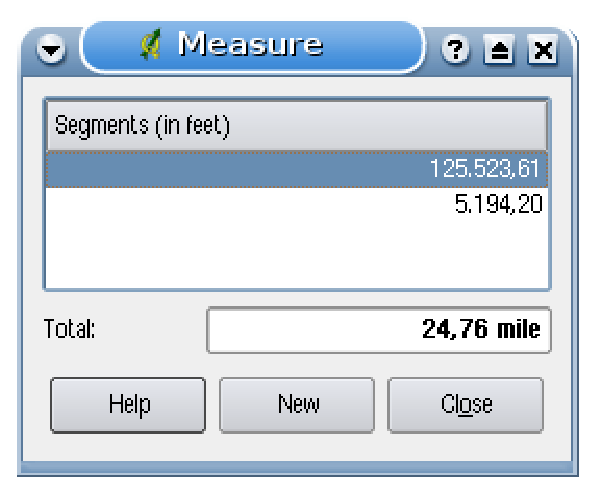
\includegraphics[clip=true, width=0.3\textwidth]{measure_line}}\goodgap
   \subfigure[Measure areas]{\label{subfig:measure_area}\includegraphics[clip=true, width=0.3\textwidth]{measure_area}}
\end{figure}

\subsection{Projects}\label{sec:projects}\index{projects}

The state of your QGIS session is considered a Project.  QGIS
works on one project at a time.  Settings are either considered
as being per-project, or as a default for new projects (see
Section \ref{subsec:gui_options}). QGIS can save the state of your 
workspace into a project file using the menu options 
\mainmenuopt{File} > \dropmenuopttwo{mActionFileSave}{Save Project}
or \mainmenuopt{File} > \dropmenuopttwo{mActionFileSaveAs}{Save Project As}.

Load saved projects into a QGIS session using 
\mainmenuopt{File} > \dropmenuopttwo{mActionFileOpen}{Open Project}
or \mainmenuopt{File} > \dropmenuopt{Open Recent Project}.
If you wish to clear your session and start fresh, choose
\mainmenuopt{File} > \dropmenuopttwo{mActionFileNew}{New Project}.
Either of these menu options will prompt you to save the existing project
if changes have been made since it was opened or last saved.

The kinds of information saved in a project file include:

\begin{itemize}
\item Layers added
\item Layer properties, including symbolization
\item Projection for the map view
\item Last viewed extent
\end{itemize}

The project file is saved in XML format, so it is possible to edit
the file outside QGIS if you know what you are doing. The file format 
was updated several times compared to earlier QGIS versions. Project files 
from older QGIS versions may not work properly anymore. To be made aware of this, 
in the \tab{General} tab under \mainmenuopt{Settings} > \dropmenuopt{Options} 
you can select \checkbox{Warn when opening a project file saved with an older 
version of QGIS}.

\subsection{Output}\label{sec:output}\index{output!save as image!print composer!quick print}
There are several ways to generate output from your QGIS session.
We have discussed one already in Section \ref{sec:projects}: saving as a project file. 
Here is a sampling of other ways to produce output files:
\begin{itemize}
\item Menu option \dropmenuopttwo{mActionSaveMapAsImage}{Save as Image} opens a
file dialog where you select the name, path and type of image (PNG or JPG format). From this
release, a world file with extension PNGW or JPGW saved in the same folder georeferences the image.
\item Menu option \dropmenuopttwo{mActionFilePrint}{Print Composer} opens a dialog 
where you can layout and print the current map canvas (see Section~\ref{label_printcomposer}).
\end{itemize}


\subsection{GUI Options}
\label{subsec:gui_options}

\includegraphics[width=0.7cm,clip=true]{mActionOptions} 
Some basic options for QGIS
can be selected using the \dialog{Options} dialog. Select the 
menu option \mainmenuopt{Settings} >
 \dropmenuopttwo{mActionOptions}{Options}. The tabs where you can 
optmize your options are:

\minisec{General Tab}

\begin{itemize}
\item \checkbox{Ask to save project changes when required}
\item \checkbox{Warn when opening a project file saved with an older version of QGIS}
\item \checkbox{Change Selection and backgroud Color}
\item Change the icon theme (choose between default, classic, gis and nkids)
\item \checkbox{Capitalise layer names in legend}
\item \checkbox{Display classification attribute names in legend}
\item \checkbox{Hide splash screen at startup}
\item \checkbox{Open attribute table in a dock window}
\item Define attribute table behavior (choose between show all features, show 
selected features and show features in current canvas)
\end{itemize}

\minisec{Rendering Tab}

\begin{itemize}
\item \checkbox{By deafult new layers added to the map should be displayed}
\item Define number of features to draw before updating the display.
\item \checkbox{Make lines appear less jagged at the expense of some drawing performance}
\item \checkbox{Fix problems with incorrectly filled polygons}
\item \checkbox{Continously redraw when dragging the legend/map divider} 
\end{itemize}

\minisec{Map tools Tab}

\begin{itemize}
\item Define Search Radius as a percentage of the map width
\item Define Ellipsoid for distance calculations
\item Define Rubberband Color for Measure Tools
\item Define Mouse wheel action (Zoom, Zoom and recenter, Zoom to mouse cursor, Nothing)
\item Define Zoom factor for wheel mouse
\end{itemize}

\minisec{Digitizing Tab}

\begin{itemize}
\item Define Rubberband Color and line width for Digitizing
\item Define default snap mode (to vertex, to segment, to vertex and segment)
\item Define default snapping tolerance in layer units
\item Define search radius for vertex edits in layer units
\item Define vertex marker style (Cross or semi transparent circle)
\end{itemize}

\minisec{CRS Tab}

\begin{itemize}
\item \checkbox{Prompt for Coordinate Reference System (CRS)}
\item \checkbox{Project wide default Coordinate Reference System (CRS) will be used}
\item \checkbox{Global default Coordinate Reference System (CRS) displayed below will be used}
\item Select global default Coordinate Reference System (CRS)
\end{itemize}

\minisec{Locale Tab}

\begin{itemize}
\item \checkbox{Overwrite system locale and use defined locale instead}
\item Information about active system locale
\end{itemize}

\minisec{Proxy Tab}

\begin{itemize}
\item \checkbox{Use proxy for web access} and define host, port, user, and password.
\item Set the \dropmenuopt{Proxy type} according to your needs
 \begin{itemize}
  \item \dropmenuopt{Default Proxy}: Proxy is determined based on the application proxy set using
  \item \dropmenuopt{Socks5Proxy}: Generic proxy for any kind of connection. Supports TCP, UDP, binding to a port (incoming connections) and authentication.
  \item \dropmenuopt{HttpProxy}: Implemented using the "CONNECT" command, supports only outgoing TCP connections; supports authentication.
  \item \dropmenuopt{HttpCachingProxy}: Implemented using normal HTTP commands, it is useful only in the context of HTTP requests
  \item \dropmenuopt{FtpCachingProxy}: Implemented using an FTP proxy, it is useful only in the context of FTP requests
 \end{itemize}
\end{itemize}

Excluding some URLs can be added to the textbox below the proxy-settings (see
fig. \ref{fig:proxy-settings}) by pressing the \button{Add}-button. After that
double-click into the just created URL-field and enter the URL you would like
to exclude from using the proxy. Obviously the button \button{Remove} removes the selected
entry.

If you need more detailed information about the different proxy-settings,
please refer to the manual of the unterlaying QT-library-documentation at
\url{http://doc.trolltech.com/4.5/qnetworkproxy.html#ProxyType-enum}.

\begin{figure}[ht]
   \begin{center}
   \caption{Proxy-settings in QGIS \nixcaption}
   \includegraphics[clip=true, width=10cm]{proxy-settings}
   \label{fig:proxy-settings}
\end{center} 
\end{figure}

\begin{Tip} \caption{\textsc{Using Proxies}}
\qgistip{Using proxies can sometimes be tricky. It is useful to 'trial and
error' the above proxy types and check if they succeed in your case.
}
\end{Tip}

You can modify the options according to your needs. Some of the changes may 
require a restart of QGIS before they will be effective.

\begin{itemize}
\item \nix{settings are saved in a texfile: \$HOME/.config/QuantumGIS/qgis.conf}
\item \osx{you can find your settings in: \$HOME/Library/Preferences/org.qgis.qgis.plist}
\item \win{settings are stored in the registry under:}
\begin{verbatim}
\\HKEY\CURRENT\USER\Software\QuantumGIS\qgis
\end{verbatim}
\end{itemize}


\subsection{Spatial Bookmarks}\label{sec:bookmarks}
\index{bookmarks}
\index{spatial bookmarks|\see{bookmarks}}

Spatial Bookmarks allow you to ``bookmark'' a geographic location and return to it later.

\subsubsection{Creating a Bookmark}
To create a bookmark:
\begin{enumerate}
\item Zoom or pan to the area of interest.
\item Select the menu option \mainmenuopt{View} > \dropmenuopt{New Bookmark} or press \keystroke{Ctrl-B}.
\item Enter a descriptive name for the bookmark (up to 255 characters).
\item Click \button{OK} to add the bookmark or \button{Cancel} to exit without adding the bookmark.
\end{enumerate}

Note that you can have multiple bookmarks with the same name.

\subsubsection{Working with Bookmarks}
To use or manage bookmarks, select the menu 
option \mainmenuopt{View} > \dropmenuopt{Show Bookmarks}.
The \dialog{Geospatial Bookmarks} dialog allows you to zoom to or delete a bookmark.
You can not edit the bookmark name or coordinates.

\subsubsection{Zooming to a Bookmark}
From the \dialog{Geospatial Bookmarks} dialog, select the desired bookmark by clicking on it, 
then click \button{Zoom To}.
You can also zoom to a bookmark by double-clicking on it.

\subsubsection{Deleting a Bookmark}
To delete a bookmark from the \dialog{Geospatial Bookmarks} dialog, click on it then click
 \button{Delete}.
Confirm your choice by clicking \button{Yes} or cancel the delete by clicking \button{No}.
